\documentclass[twoside]{book}

% Packages required by doxygen
\usepackage{fixltx2e}
\usepackage{calc}
\usepackage{doxygen}
\usepackage[export]{adjustbox} % also loads graphicx
\usepackage{graphicx}
\usepackage[utf8]{inputenc}
\usepackage{makeidx}
\usepackage{multicol}
\usepackage{multirow}
\PassOptionsToPackage{warn}{textcomp}
\usepackage{textcomp}
\usepackage[nointegrals]{wasysym}
\usepackage[table]{xcolor}

% Font selection
\usepackage[T1]{fontenc}
\usepackage[scaled=.90]{helvet}
\usepackage{courier}
\usepackage{amssymb}
\usepackage{sectsty}
\renewcommand{\familydefault}{\sfdefault}
\allsectionsfont{%
  \fontseries{bc}\selectfont%
  \color{darkgray}%
}
\renewcommand{\DoxyLabelFont}{%
  \fontseries{bc}\selectfont%
  \color{darkgray}%
}
\newcommand{\+}{\discretionary{\mbox{\scriptsize$\hookleftarrow$}}{}{}}

% Page & text layout
\usepackage{geometry}
\geometry{%
  a4paper,%
  top=2.5cm,%
  bottom=2.5cm,%
  left=2.5cm,%
  right=2.5cm%
}
\tolerance=750
\hfuzz=15pt
\hbadness=750
\setlength{\emergencystretch}{15pt}
\setlength{\parindent}{0cm}
\setlength{\parskip}{3ex plus 2ex minus 2ex}
\makeatletter
\renewcommand{\paragraph}{%
  \@startsection{paragraph}{4}{0ex}{-1.0ex}{1.0ex}{%
    \normalfont\normalsize\bfseries\SS@parafont%
  }%
}
\renewcommand{\subparagraph}{%
  \@startsection{subparagraph}{5}{0ex}{-1.0ex}{1.0ex}{%
    \normalfont\normalsize\bfseries\SS@subparafont%
  }%
}
\makeatother

% Headers & footers
\usepackage{fancyhdr}
\pagestyle{fancyplain}
\fancyhead[LE]{\fancyplain{}{\bfseries\thepage}}
\fancyhead[CE]{\fancyplain{}{}}
\fancyhead[RE]{\fancyplain{}{\bfseries\leftmark}}
\fancyhead[LO]{\fancyplain{}{\bfseries\rightmark}}
\fancyhead[CO]{\fancyplain{}{}}
\fancyhead[RO]{\fancyplain{}{\bfseries\thepage}}
\fancyfoot[LE]{\fancyplain{}{}}
\fancyfoot[CE]{\fancyplain{}{}}
\fancyfoot[RE]{\fancyplain{}{\bfseries\scriptsize Generated by Doxygen }}
\fancyfoot[LO]{\fancyplain{}{\bfseries\scriptsize Generated by Doxygen }}
\fancyfoot[CO]{\fancyplain{}{}}
\fancyfoot[RO]{\fancyplain{}{}}
\renewcommand{\footrulewidth}{0.4pt}
\renewcommand{\chaptermark}[1]{%
  \markboth{#1}{}%
}
\renewcommand{\sectionmark}[1]{%
  \markright{\thesection\ #1}%
}

% Indices & bibliography
\usepackage{natbib}
\usepackage[titles]{tocloft}
\setcounter{tocdepth}{3}
\setcounter{secnumdepth}{5}
\makeindex

% Hyperlinks (required, but should be loaded last)
\usepackage{ifpdf}
\ifpdf
  \usepackage[pdftex,pagebackref=true]{hyperref}
\else
  \usepackage[ps2pdf,pagebackref=true]{hyperref}
\fi
\hypersetup{%
  colorlinks=true,%
  linkcolor=blue,%
  citecolor=blue,%
  unicode%
}

% Custom commands
\newcommand{\clearemptydoublepage}{%
  \newpage{\pagestyle{empty}\cleardoublepage}%
}

\usepackage{caption}
\captionsetup{labelsep=space,justification=centering,font={bf},singlelinecheck=off,skip=4pt,position=top}

%===== C O N T E N T S =====

\begin{document}

% Titlepage & ToC
\hypersetup{pageanchor=false,
             bookmarksnumbered=true,
             pdfencoding=unicode
            }
\pagenumbering{alph}
\begin{titlepage}
\vspace*{7cm}
\begin{center}%
{\Large Core Resource Access Monitor }\\
\vspace*{1cm}
{\large Generated by Doxygen 1.8.14}\\
\end{center}
\end{titlepage}
\clearemptydoublepage
\pagenumbering{roman}
\tableofcontents
\clearemptydoublepage
\pagenumbering{arabic}
\hypersetup{pageanchor=true}

%--- Begin generated contents ---
\chapter{R\+E\+A\+D\+ME}
\label{md_README}
\Hypertarget{md_README}
\href{https://api.travis-ci.org/symbiote-h2020/CoreResourceAccessMonitor}{\tt } \href{https://codecov.io/github/symbiote-h2020/CoreResourceAccessMonitor/branch/staging}{\tt }

\section*{Core\+Resource\+Access\+Monitor}
\chapter{Hierarchical Index}
\section{Class Hierarchy}
This inheritance list is sorted roughly, but not completely, alphabetically\+:\begin{DoxyCompactList}
\item \contentsline{section}{eu.\+h2020.\+symbiote.\+Core\+Resource\+Access\+Monitor\+Application}{\pageref{classeu_1_1h2020_1_1symbiote_1_1CoreResourceAccessMonitorApplication}}{}
\item \contentsline{section}{eu.\+h2020.\+symbiote.\+model.\+Location}{\pageref{classeu_1_1h2020_1_1symbiote_1_1model_1_1Location}}{}
\item \contentsline{section}{eu.\+h2020.\+symbiote.\+model.\+Platform}{\pageref{classeu_1_1h2020_1_1symbiote_1_1model_1_1Platform}}{}
\item \contentsline{section}{eu.\+h2020.\+symbiote.\+repository.\+Repository\+Manager}{\pageref{classeu_1_1h2020_1_1symbiote_1_1repository_1_1RepositoryManager}}{}
\item \contentsline{section}{eu.\+h2020.\+symbiote.\+model.\+Resource}{\pageref{classeu_1_1h2020_1_1symbiote_1_1model_1_1Resource}}{}
\item \contentsline{section}{eu.\+h2020.\+symbiote.\+messaging.\+Rpc\+Server}{\pageref{classeu_1_1h2020_1_1symbiote_1_1messaging_1_1RpcServer}}{}
\item Amqp\+Reject\+And\+Dont\+Requeue\+Exception\begin{DoxyCompactList}
\item \contentsline{section}{eu.\+h2020.\+symbiote.\+exception.\+Entity\+Not\+Found\+Exception}{\pageref{classeu_1_1h2020_1_1symbiote_1_1exception_1_1EntityNotFoundException}}{}
\end{DoxyCompactList}
\item Mongo\+Repository\begin{DoxyCompactList}
\item \contentsline{section}{eu.\+h2020.\+symbiote.\+repository.\+Platform\+Repository}{\pageref{interfaceeu_1_1h2020_1_1symbiote_1_1repository_1_1PlatformRepository}}{}
\item \contentsline{section}{eu.\+h2020.\+symbiote.\+repository.\+Resource\+Repository}{\pageref{interfaceeu_1_1h2020_1_1symbiote_1_1repository_1_1ResourceRepository}}{}
\end{DoxyCompactList}
\end{DoxyCompactList}

\chapter{Class Index}
\section{Class List}
Here are the classes, structs, unions and interfaces with brief descriptions\+:\begin{DoxyCompactList}
\item\contentsline{section}{\hyperlink{classeu_1_1h2020_1_1symbiote_1_1CoreResourceAccessMonitorApplication}{eu.\+h2020.\+symbiote.\+Core\+Resource\+Access\+Monitor\+Application} }{\pageref{classeu_1_1h2020_1_1symbiote_1_1CoreResourceAccessMonitorApplication}}{}
\item\contentsline{section}{\hyperlink{classeu_1_1h2020_1_1symbiote_1_1exception_1_1EntityNotFoundException}{eu.\+h2020.\+symbiote.\+exception.\+Entity\+Not\+Found\+Exception} }{\pageref{classeu_1_1h2020_1_1symbiote_1_1exception_1_1EntityNotFoundException}}{}
\item\contentsline{section}{\hyperlink{classeu_1_1h2020_1_1symbiote_1_1model_1_1Location}{eu.\+h2020.\+symbiote.\+model.\+Location} }{\pageref{classeu_1_1h2020_1_1symbiote_1_1model_1_1Location}}{}
\item\contentsline{section}{\hyperlink{classeu_1_1h2020_1_1symbiote_1_1model_1_1Platform}{eu.\+h2020.\+symbiote.\+model.\+Platform} }{\pageref{classeu_1_1h2020_1_1symbiote_1_1model_1_1Platform}}{}
\item\contentsline{section}{\hyperlink{interfaceeu_1_1h2020_1_1symbiote_1_1repository_1_1PlatformRepository}{eu.\+h2020.\+symbiote.\+repository.\+Platform\+Repository} }{\pageref{interfaceeu_1_1h2020_1_1symbiote_1_1repository_1_1PlatformRepository}}{}
\item\contentsline{section}{\hyperlink{classeu_1_1h2020_1_1symbiote_1_1repository_1_1RepositoryManager}{eu.\+h2020.\+symbiote.\+repository.\+Repository\+Manager} }{\pageref{classeu_1_1h2020_1_1symbiote_1_1repository_1_1RepositoryManager}}{}
\item\contentsline{section}{\hyperlink{classeu_1_1h2020_1_1symbiote_1_1model_1_1Resource}{eu.\+h2020.\+symbiote.\+model.\+Resource} }{\pageref{classeu_1_1h2020_1_1symbiote_1_1model_1_1Resource}}{}
\item\contentsline{section}{\hyperlink{interfaceeu_1_1h2020_1_1symbiote_1_1repository_1_1ResourceRepository}{eu.\+h2020.\+symbiote.\+repository.\+Resource\+Repository} }{\pageref{interfaceeu_1_1h2020_1_1symbiote_1_1repository_1_1ResourceRepository}}{}
\item\contentsline{section}{\hyperlink{classeu_1_1h2020_1_1symbiote_1_1messaging_1_1RpcServer}{eu.\+h2020.\+symbiote.\+messaging.\+Rpc\+Server} }{\pageref{classeu_1_1h2020_1_1symbiote_1_1messaging_1_1RpcServer}}{}
\end{DoxyCompactList}

\chapter{Class Documentation}
\hypertarget{classeu_1_1h2020_1_1symbiote_1_1CoreResourceAccessMonitorApplication}{}\section{eu.\+h2020.\+symbiote.\+Core\+Resource\+Access\+Monitor\+Application Class Reference}
\label{classeu_1_1h2020_1_1symbiote_1_1CoreResourceAccessMonitorApplication}\index{eu.\+h2020.\+symbiote.\+Core\+Resource\+Access\+Monitor\+Application@{eu.\+h2020.\+symbiote.\+Core\+Resource\+Access\+Monitor\+Application}}


Collaboration diagram for eu.\+h2020.\+symbiote.\+Core\+Resource\+Access\+Monitor\+Application\+:
\nopagebreak
\begin{figure}[H]
\begin{center}
\leavevmode
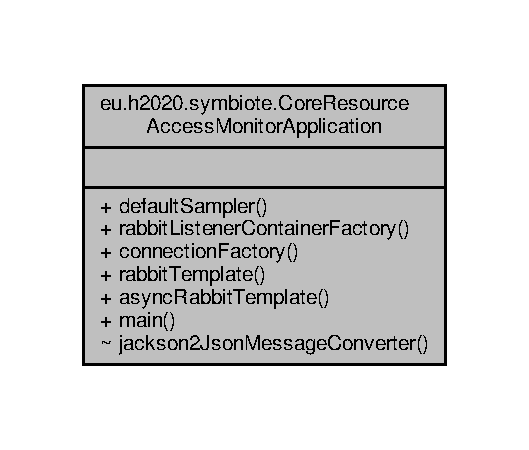
\includegraphics[width=254pt]{classeu_1_1h2020_1_1symbiote_1_1CoreResourceAccessMonitorApplication__coll__graph}
\end{center}
\end{figure}
\subsection*{Public Member Functions}
\begin{DoxyCompactItemize}
\item 
\mbox{\Hypertarget{classeu_1_1h2020_1_1symbiote_1_1CoreResourceAccessMonitorApplication_a77cd3f3ac1cd8247d43679a7c3d67a0b}\label{classeu_1_1h2020_1_1symbiote_1_1CoreResourceAccessMonitorApplication_a77cd3f3ac1cd8247d43679a7c3d67a0b}} 
Always\+Sampler {\bfseries default\+Sampler} ()
\item 
\mbox{\Hypertarget{classeu_1_1h2020_1_1symbiote_1_1CoreResourceAccessMonitorApplication_a511d4f9d77b66d6c647b68fb1ad3e797}\label{classeu_1_1h2020_1_1symbiote_1_1CoreResourceAccessMonitorApplication_a511d4f9d77b66d6c647b68fb1ad3e797}} 
Simple\+Rabbit\+Listener\+Container\+Factory {\bfseries rabbit\+Listener\+Container\+Factory} (Connection\+Factory connection\+Factory)
\item 
\mbox{\Hypertarget{classeu_1_1h2020_1_1symbiote_1_1CoreResourceAccessMonitorApplication_a14fb66e3a9c4ef134ef0bb31aaaafbdf}\label{classeu_1_1h2020_1_1symbiote_1_1CoreResourceAccessMonitorApplication_a14fb66e3a9c4ef134ef0bb31aaaafbdf}} 
Connection\+Factory {\bfseries connection\+Factory} ()  throws Exception 
\item 
\mbox{\Hypertarget{classeu_1_1h2020_1_1symbiote_1_1CoreResourceAccessMonitorApplication_a4b518b81cb1ef9ba85e823abd4ec4fd6}\label{classeu_1_1h2020_1_1symbiote_1_1CoreResourceAccessMonitorApplication_a4b518b81cb1ef9ba85e823abd4ec4fd6}} 
Rabbit\+Template {\bfseries rabbit\+Template} (Connection\+Factory connection\+Factory, Jackson2\+Json\+Message\+Converter jackson2\+Json\+Message\+Converter)
\item 
Async\+Rabbit\+Template \hyperlink{classeu_1_1h2020_1_1symbiote_1_1CoreResourceAccessMonitorApplication_a5ddd9256ae88e6362a7e76b640d24f50}{async\+Rabbit\+Template} (Rabbit\+Template rabbit\+Template)
\end{DoxyCompactItemize}
\subsection*{Static Public Member Functions}
\begin{DoxyCompactItemize}
\item 
\mbox{\Hypertarget{classeu_1_1h2020_1_1symbiote_1_1CoreResourceAccessMonitorApplication_adbc7e65218ff32b0690b9114cda8aad3}\label{classeu_1_1h2020_1_1symbiote_1_1CoreResourceAccessMonitorApplication_adbc7e65218ff32b0690b9114cda8aad3}} 
static void {\bfseries main} (String\mbox{[}$\,$\mbox{]} args)
\end{DoxyCompactItemize}


\subsection{Member Function Documentation}
\mbox{\Hypertarget{classeu_1_1h2020_1_1symbiote_1_1CoreResourceAccessMonitorApplication_a5ddd9256ae88e6362a7e76b640d24f50}\label{classeu_1_1h2020_1_1symbiote_1_1CoreResourceAccessMonitorApplication_a5ddd9256ae88e6362a7e76b640d24f50}} 
\index{eu\+::h2020\+::symbiote\+::\+Core\+Resource\+Access\+Monitor\+Application@{eu\+::h2020\+::symbiote\+::\+Core\+Resource\+Access\+Monitor\+Application}!async\+Rabbit\+Template@{async\+Rabbit\+Template}}
\index{async\+Rabbit\+Template@{async\+Rabbit\+Template}!eu\+::h2020\+::symbiote\+::\+Core\+Resource\+Access\+Monitor\+Application@{eu\+::h2020\+::symbiote\+::\+Core\+Resource\+Access\+Monitor\+Application}}
\subsubsection{\texorpdfstring{async\+Rabbit\+Template()}{asyncRabbitTemplate()}}
{\footnotesize\ttfamily Async\+Rabbit\+Template eu.\+h2020.\+symbiote.\+Core\+Resource\+Access\+Monitor\+Application.\+async\+Rabbit\+Template (\begin{DoxyParamCaption}\item[{Rabbit\+Template}]{rabbit\+Template }\end{DoxyParamCaption})}

The following Async\+Rabbit\+Template constructor uses \char`\"{}\+Direct reply\+To\char`\"{} for replies.

The documentation for this class was generated from the following file\+:\begin{DoxyCompactItemize}
\item 
src/main/java/eu/h2020/symbiote/Core\+Resource\+Access\+Monitor\+Application.\+java\end{DoxyCompactItemize}

\hypertarget{classeu_1_1h2020_1_1symbiote_1_1exception_1_1EntityNotFoundException}{}\section{eu.\+h2020.\+symbiote.\+exception.\+Entity\+Not\+Found\+Exception Class Reference}
\label{classeu_1_1h2020_1_1symbiote_1_1exception_1_1EntityNotFoundException}\index{eu.\+h2020.\+symbiote.\+exception.\+Entity\+Not\+Found\+Exception@{eu.\+h2020.\+symbiote.\+exception.\+Entity\+Not\+Found\+Exception}}


Inheritance diagram for eu.\+h2020.\+symbiote.\+exception.\+Entity\+Not\+Found\+Exception\+:
\nopagebreak
\begin{figure}[H]
\begin{center}
\leavevmode
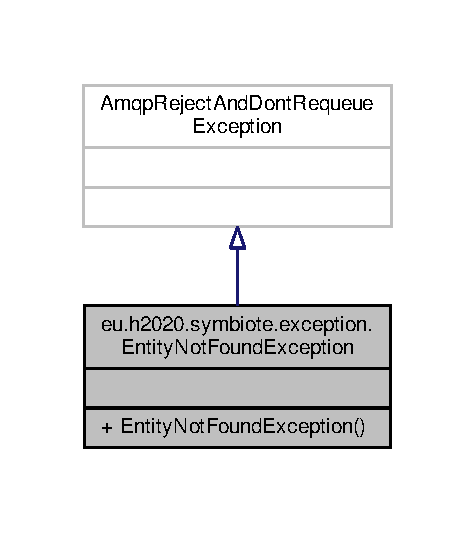
\includegraphics[width=228pt]{classeu_1_1h2020_1_1symbiote_1_1exception_1_1EntityNotFoundException__inherit__graph}
\end{center}
\end{figure}


Collaboration diagram for eu.\+h2020.\+symbiote.\+exception.\+Entity\+Not\+Found\+Exception\+:
\nopagebreak
\begin{figure}[H]
\begin{center}
\leavevmode
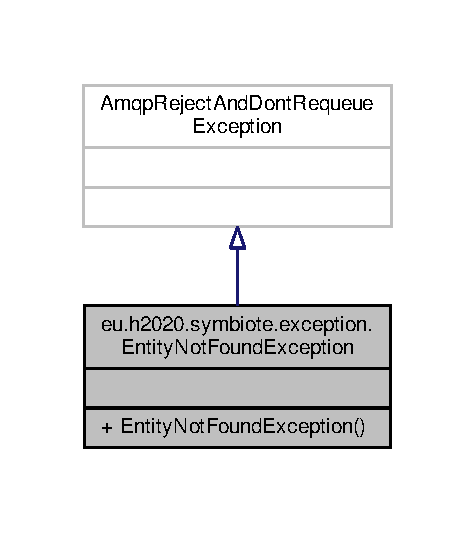
\includegraphics[width=228pt]{classeu_1_1h2020_1_1symbiote_1_1exception_1_1EntityNotFoundException__coll__graph}
\end{center}
\end{figure}
\subsection*{Public Member Functions}
\begin{DoxyCompactItemize}
\item 
\mbox{\Hypertarget{classeu_1_1h2020_1_1symbiote_1_1exception_1_1EntityNotFoundException_a3ac61b38a6d41a71faf6adc95b9d1d79}\label{classeu_1_1h2020_1_1symbiote_1_1exception_1_1EntityNotFoundException_a3ac61b38a6d41a71faf6adc95b9d1d79}} 
{\bfseries Entity\+Not\+Found\+Exception} (String message)
\end{DoxyCompactItemize}


\subsection{Detailed Description}
\begin{DoxyAuthor}{Author}
Vasileios Glykantzis \href{mailto:vasgl@intracom-telecom.com}{\tt vasgl@intracom-\/telecom.\+com} 
\end{DoxyAuthor}


The documentation for this class was generated from the following file\+:\begin{DoxyCompactItemize}
\item 
src/main/java/eu/h2020/symbiote/exception/Entity\+Not\+Found\+Exception.\+java\end{DoxyCompactItemize}

\hypertarget{classeu_1_1h2020_1_1symbiote_1_1model_1_1Location}{}\section{eu.\+h2020.\+symbiote.\+model.\+Location Class Reference}
\label{classeu_1_1h2020_1_1symbiote_1_1model_1_1Location}\index{eu.\+h2020.\+symbiote.\+model.\+Location@{eu.\+h2020.\+symbiote.\+model.\+Location}}


Collaboration diagram for eu.\+h2020.\+symbiote.\+model.\+Location\+:
\nopagebreak
\begin{figure}[H]
\begin{center}
\leavevmode
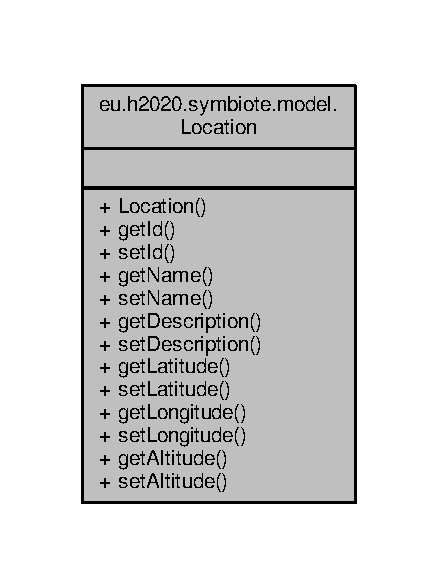
\includegraphics[width=210pt]{classeu_1_1h2020_1_1symbiote_1_1model_1_1Location__coll__graph}
\end{center}
\end{figure}
\subsection*{Public Member Functions}
\begin{DoxyCompactItemize}
\item 
\mbox{\Hypertarget{classeu_1_1h2020_1_1symbiote_1_1model_1_1Location_a98a3b93d177deb7b9630c5e37547d80d}\label{classeu_1_1h2020_1_1symbiote_1_1model_1_1Location_a98a3b93d177deb7b9630c5e37547d80d}} 
String {\bfseries get\+Id} ()
\item 
\mbox{\Hypertarget{classeu_1_1h2020_1_1symbiote_1_1model_1_1Location_a308f71eeeed57f22b5996da217028d29}\label{classeu_1_1h2020_1_1symbiote_1_1model_1_1Location_a308f71eeeed57f22b5996da217028d29}} 
void {\bfseries set\+Id} (String id)
\item 
\mbox{\Hypertarget{classeu_1_1h2020_1_1symbiote_1_1model_1_1Location_a78e563a2622952f37da6f571932afa23}\label{classeu_1_1h2020_1_1symbiote_1_1model_1_1Location_a78e563a2622952f37da6f571932afa23}} 
String {\bfseries get\+Name} ()
\item 
\mbox{\Hypertarget{classeu_1_1h2020_1_1symbiote_1_1model_1_1Location_a67ddf61270deeb669ebcdce9b9ead998}\label{classeu_1_1h2020_1_1symbiote_1_1model_1_1Location_a67ddf61270deeb669ebcdce9b9ead998}} 
void {\bfseries set\+Name} (String name)
\item 
\mbox{\Hypertarget{classeu_1_1h2020_1_1symbiote_1_1model_1_1Location_accf0bb0ab10306a962e09fc32c8d821c}\label{classeu_1_1h2020_1_1symbiote_1_1model_1_1Location_accf0bb0ab10306a962e09fc32c8d821c}} 
String {\bfseries get\+Description} ()
\item 
\mbox{\Hypertarget{classeu_1_1h2020_1_1symbiote_1_1model_1_1Location_a45d3f8f4397791af93669578501a43bf}\label{classeu_1_1h2020_1_1symbiote_1_1model_1_1Location_a45d3f8f4397791af93669578501a43bf}} 
void {\bfseries set\+Description} (String description)
\item 
\mbox{\Hypertarget{classeu_1_1h2020_1_1symbiote_1_1model_1_1Location_a40812abe56323ccb3e65d1309d2d55e4}\label{classeu_1_1h2020_1_1symbiote_1_1model_1_1Location_a40812abe56323ccb3e65d1309d2d55e4}} 
double {\bfseries get\+Latitude} ()
\item 
\mbox{\Hypertarget{classeu_1_1h2020_1_1symbiote_1_1model_1_1Location_a26b8aab258d4422bd5fc64d7a512b685}\label{classeu_1_1h2020_1_1symbiote_1_1model_1_1Location_a26b8aab258d4422bd5fc64d7a512b685}} 
void {\bfseries set\+Latitude} (double latitude)
\item 
\mbox{\Hypertarget{classeu_1_1h2020_1_1symbiote_1_1model_1_1Location_afe9ac4993b9dbcc9350e2667e279d39b}\label{classeu_1_1h2020_1_1symbiote_1_1model_1_1Location_afe9ac4993b9dbcc9350e2667e279d39b}} 
double {\bfseries get\+Longitude} ()
\item 
\mbox{\Hypertarget{classeu_1_1h2020_1_1symbiote_1_1model_1_1Location_a6bc9a04947915ea52001bccbcba0849e}\label{classeu_1_1h2020_1_1symbiote_1_1model_1_1Location_a6bc9a04947915ea52001bccbcba0849e}} 
void {\bfseries set\+Longitude} (double longitude)
\item 
\mbox{\Hypertarget{classeu_1_1h2020_1_1symbiote_1_1model_1_1Location_a333c37abcd3c9ea766ca5ec6dddd5e3a}\label{classeu_1_1h2020_1_1symbiote_1_1model_1_1Location_a333c37abcd3c9ea766ca5ec6dddd5e3a}} 
double {\bfseries get\+Altitude} ()
\item 
\mbox{\Hypertarget{classeu_1_1h2020_1_1symbiote_1_1model_1_1Location_ac2fc6d59229ad7253416f2fdf650675d}\label{classeu_1_1h2020_1_1symbiote_1_1model_1_1Location_ac2fc6d59229ad7253416f2fdf650675d}} 
void {\bfseries set\+Altitude} (double altitude)
\end{DoxyCompactItemize}


\subsection{Detailed Description}
Created by jawora on 21.\+12.\+16. 

The documentation for this class was generated from the following file\+:\begin{DoxyCompactItemize}
\item 
src/main/java/eu/h2020/symbiote/model/Location.\+java\end{DoxyCompactItemize}

\hypertarget{classeu_1_1h2020_1_1symbiote_1_1model_1_1Platform}{}\section{eu.\+h2020.\+symbiote.\+model.\+Platform Class Reference}
\label{classeu_1_1h2020_1_1symbiote_1_1model_1_1Platform}\index{eu.\+h2020.\+symbiote.\+model.\+Platform@{eu.\+h2020.\+symbiote.\+model.\+Platform}}


Collaboration diagram for eu.\+h2020.\+symbiote.\+model.\+Platform\+:
\nopagebreak
\begin{figure}[H]
\begin{center}
\leavevmode
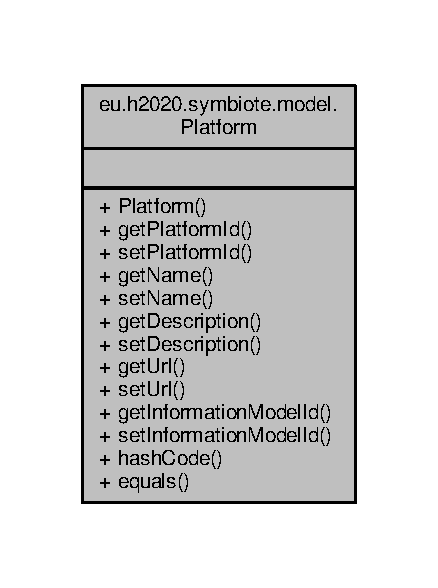
\includegraphics[width=210pt]{classeu_1_1h2020_1_1symbiote_1_1model_1_1Platform__coll__graph}
\end{center}
\end{figure}
\subsection*{Public Member Functions}
\begin{DoxyCompactItemize}
\item 
\mbox{\Hypertarget{classeu_1_1h2020_1_1symbiote_1_1model_1_1Platform_a2a09b94af05846adcf58f6405f0b1fdc}\label{classeu_1_1h2020_1_1symbiote_1_1model_1_1Platform_a2a09b94af05846adcf58f6405f0b1fdc}} 
String {\bfseries get\+Platform\+Id} ()
\item 
\mbox{\Hypertarget{classeu_1_1h2020_1_1symbiote_1_1model_1_1Platform_a3d9e886790d506f713e997f3c587e8ac}\label{classeu_1_1h2020_1_1symbiote_1_1model_1_1Platform_a3d9e886790d506f713e997f3c587e8ac}} 
void {\bfseries set\+Platform\+Id} (String platform\+Id)
\item 
\mbox{\Hypertarget{classeu_1_1h2020_1_1symbiote_1_1model_1_1Platform_a9d39e85c470888c7043448f2eb059325}\label{classeu_1_1h2020_1_1symbiote_1_1model_1_1Platform_a9d39e85c470888c7043448f2eb059325}} 
String {\bfseries get\+Name} ()
\item 
\mbox{\Hypertarget{classeu_1_1h2020_1_1symbiote_1_1model_1_1Platform_af4d5506c08659b3d71dcc8bf69c743ce}\label{classeu_1_1h2020_1_1symbiote_1_1model_1_1Platform_af4d5506c08659b3d71dcc8bf69c743ce}} 
void {\bfseries set\+Name} (String name)
\item 
\mbox{\Hypertarget{classeu_1_1h2020_1_1symbiote_1_1model_1_1Platform_ad4a8d6cbb5ed57e241f783c512f052d9}\label{classeu_1_1h2020_1_1symbiote_1_1model_1_1Platform_ad4a8d6cbb5ed57e241f783c512f052d9}} 
String {\bfseries get\+Description} ()
\item 
\mbox{\Hypertarget{classeu_1_1h2020_1_1symbiote_1_1model_1_1Platform_a9ec81f09b9fcd25ae264618591992cb2}\label{classeu_1_1h2020_1_1symbiote_1_1model_1_1Platform_a9ec81f09b9fcd25ae264618591992cb2}} 
void {\bfseries set\+Description} (String description)
\item 
\mbox{\Hypertarget{classeu_1_1h2020_1_1symbiote_1_1model_1_1Platform_a4ca440b89e37c323dcb812ef07cfb66a}\label{classeu_1_1h2020_1_1symbiote_1_1model_1_1Platform_a4ca440b89e37c323dcb812ef07cfb66a}} 
String {\bfseries get\+Url} ()
\item 
\mbox{\Hypertarget{classeu_1_1h2020_1_1symbiote_1_1model_1_1Platform_ac4d39a74475da2c2318cfd5e3667a5a1}\label{classeu_1_1h2020_1_1symbiote_1_1model_1_1Platform_ac4d39a74475da2c2318cfd5e3667a5a1}} 
void {\bfseries set\+Url} (String url)
\item 
\mbox{\Hypertarget{classeu_1_1h2020_1_1symbiote_1_1model_1_1Platform_a799a5bb8e0665457c4b8bfd2b34c9b3c}\label{classeu_1_1h2020_1_1symbiote_1_1model_1_1Platform_a799a5bb8e0665457c4b8bfd2b34c9b3c}} 
String {\bfseries get\+Information\+Model\+Id} ()
\item 
\mbox{\Hypertarget{classeu_1_1h2020_1_1symbiote_1_1model_1_1Platform_ae3e1cb93bcb289d575f215990d7e9499}\label{classeu_1_1h2020_1_1symbiote_1_1model_1_1Platform_ae3e1cb93bcb289d575f215990d7e9499}} 
void {\bfseries set\+Information\+Model\+Id} (String information\+Model\+Id)
\item 
\mbox{\Hypertarget{classeu_1_1h2020_1_1symbiote_1_1model_1_1Platform_a3b85d6919db55e5a8584a909a4599953}\label{classeu_1_1h2020_1_1symbiote_1_1model_1_1Platform_a3b85d6919db55e5a8584a909a4599953}} 
int {\bfseries hash\+Code} ()
\item 
\mbox{\Hypertarget{classeu_1_1h2020_1_1symbiote_1_1model_1_1Platform_ab00da56375115817b0594f8865667d30}\label{classeu_1_1h2020_1_1symbiote_1_1model_1_1Platform_ab00da56375115817b0594f8865667d30}} 
boolean {\bfseries equals} (Object obj)
\end{DoxyCompactItemize}


\subsection{Detailed Description}
Created by mateuszl on 09.\+01.\+2017. 

The documentation for this class was generated from the following file\+:\begin{DoxyCompactItemize}
\item 
src/main/java/eu/h2020/symbiote/model/Platform.\+java\end{DoxyCompactItemize}

\hypertarget{interfaceeu_1_1h2020_1_1symbiote_1_1repository_1_1PlatformRepository}{}\section{eu.\+h2020.\+symbiote.\+repository.\+Platform\+Repository Interface Reference}
\label{interfaceeu_1_1h2020_1_1symbiote_1_1repository_1_1PlatformRepository}\index{eu.\+h2020.\+symbiote.\+repository.\+Platform\+Repository@{eu.\+h2020.\+symbiote.\+repository.\+Platform\+Repository}}


Inheritance diagram for eu.\+h2020.\+symbiote.\+repository.\+Platform\+Repository\+:
\nopagebreak
\begin{figure}[H]
\begin{center}
\leavevmode
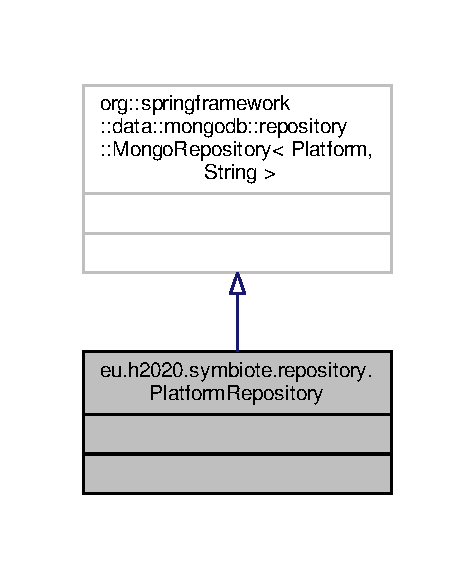
\includegraphics[width=228pt]{interfaceeu_1_1h2020_1_1symbiote_1_1repository_1_1PlatformRepository__inherit__graph}
\end{center}
\end{figure}


Collaboration diagram for eu.\+h2020.\+symbiote.\+repository.\+Platform\+Repository\+:
\nopagebreak
\begin{figure}[H]
\begin{center}
\leavevmode
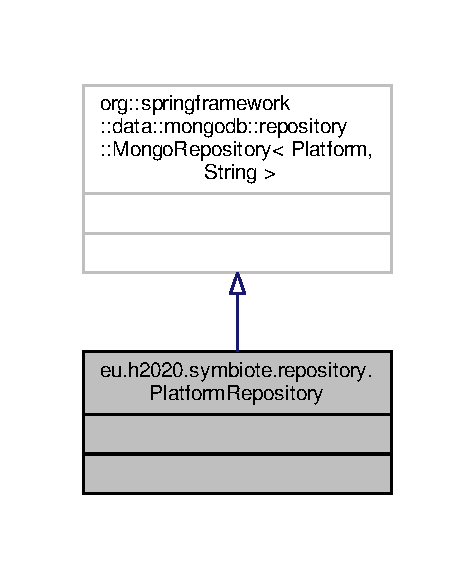
\includegraphics[width=228pt]{interfaceeu_1_1h2020_1_1symbiote_1_1repository_1_1PlatformRepository__coll__graph}
\end{center}
\end{figure}


\subsection{Detailed Description}
Created by mateuszl on 22.\+09.\+2016. 

The documentation for this interface was generated from the following file\+:\begin{DoxyCompactItemize}
\item 
src/main/java/eu/h2020/symbiote/repository/Platform\+Repository.\+java\end{DoxyCompactItemize}

\hypertarget{classeu_1_1h2020_1_1symbiote_1_1repository_1_1RepositoryManager}{}\section{eu.\+h2020.\+symbiote.\+repository.\+Repository\+Manager Class Reference}
\label{classeu_1_1h2020_1_1symbiote_1_1repository_1_1RepositoryManager}\index{eu.\+h2020.\+symbiote.\+repository.\+Repository\+Manager@{eu.\+h2020.\+symbiote.\+repository.\+Repository\+Manager}}


Collaboration diagram for eu.\+h2020.\+symbiote.\+repository.\+Repository\+Manager\+:
\nopagebreak
\begin{figure}[H]
\begin{center}
\leavevmode
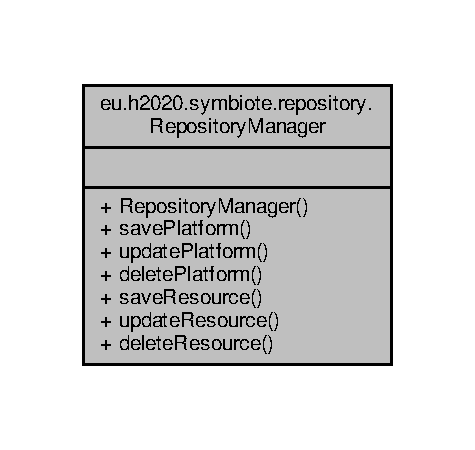
\includegraphics[width=228pt]{classeu_1_1h2020_1_1symbiote_1_1repository_1_1RepositoryManager__coll__graph}
\end{center}
\end{figure}
\subsection*{Public Member Functions}
\begin{DoxyCompactItemize}
\item 
\mbox{\Hypertarget{classeu_1_1h2020_1_1symbiote_1_1repository_1_1RepositoryManager_a75d70aebe267b3b304ef708547996e5a}\label{classeu_1_1h2020_1_1symbiote_1_1repository_1_1RepositoryManager_a75d70aebe267b3b304ef708547996e5a}} 
{\bfseries Repository\+Manager} (\hyperlink{interfaceeu_1_1h2020_1_1symbiote_1_1repository_1_1PlatformRepository}{Platform\+Repository} platform\+Repository, \hyperlink{interfaceeu_1_1h2020_1_1symbiote_1_1repository_1_1ResourceRepository}{Resource\+Repository} resource\+Repository)
\end{DoxyCompactItemize}
\subsection*{Static Public Member Functions}
\begin{DoxyCompactItemize}
\item 
static void \hyperlink{classeu_1_1h2020_1_1symbiote_1_1repository_1_1RepositoryManager_a496929533495f38ece4f1c5c8bee4bb4}{save\+Platform} (\hyperlink{classeu_1_1h2020_1_1symbiote_1_1model_1_1Platform}{Platform} platform)
\item 
static void \hyperlink{classeu_1_1h2020_1_1symbiote_1_1repository_1_1RepositoryManager_ab40bbdbdd46c6db2eaa59a615c38cfd0}{update\+Platform} (\hyperlink{classeu_1_1h2020_1_1symbiote_1_1model_1_1Platform}{Platform} platform)  throws Entity\+Not\+Found\+Exception 
\item 
static void \hyperlink{classeu_1_1h2020_1_1symbiote_1_1repository_1_1RepositoryManager_ab7f93e37749010ead2699037d54c4b0d}{delete\+Platform} (\hyperlink{classeu_1_1h2020_1_1symbiote_1_1model_1_1Platform}{Platform} platform)  throws Entity\+Not\+Found\+Exception 
\item 
static void \hyperlink{classeu_1_1h2020_1_1symbiote_1_1repository_1_1RepositoryManager_a82eb799665755be27795dafdfe90e0b3}{save\+Resource} (\hyperlink{classeu_1_1h2020_1_1symbiote_1_1model_1_1Resource}{Resource} resource)  throws Entity\+Not\+Found\+Exception 
\item 
static void \hyperlink{classeu_1_1h2020_1_1symbiote_1_1repository_1_1RepositoryManager_a49626e0b688780c44cac19cf9e3f1a51}{update\+Resource} (\hyperlink{classeu_1_1h2020_1_1symbiote_1_1model_1_1Resource}{Resource} resource)  throws Entity\+Not\+Found\+Exception 
\item 
static void \hyperlink{classeu_1_1h2020_1_1symbiote_1_1repository_1_1RepositoryManager_aa943334bc33d9e5b9a81978558caba89}{delete\+Resource} (\hyperlink{classeu_1_1h2020_1_1symbiote_1_1model_1_1Resource}{Resource} resource)  throws Entity\+Not\+Found\+Exception 
\end{DoxyCompactItemize}


\subsection{Detailed Description}
\subsection*{Repository Manager for saving platform and resource information}

This listens to platform and resource events advertised by registry and saves them to the local Mongo database.

\begin{DoxyAuthor}{Author}
Tilemachos Pechlivanoglou \href{mailto:tipech@intracom-telecom.com}{\tt tipech@intracom-\/telecom.\+com} 

Vasileios Glykantzis \href{mailto:vasgl@intracom-telecom.com}{\tt vasgl@intracom-\/telecom.\+com} 
\end{DoxyAuthor}
\begin{DoxyVersion}{Version}
1.\+0 
\end{DoxyVersion}
\begin{DoxySince}{Since}
2017-\/01-\/26 
\end{DoxySince}


\subsection{Member Function Documentation}
\mbox{\Hypertarget{classeu_1_1h2020_1_1symbiote_1_1repository_1_1RepositoryManager_ab7f93e37749010ead2699037d54c4b0d}\label{classeu_1_1h2020_1_1symbiote_1_1repository_1_1RepositoryManager_ab7f93e37749010ead2699037d54c4b0d}} 
\index{eu\+::h2020\+::symbiote\+::repository\+::\+Repository\+Manager@{eu\+::h2020\+::symbiote\+::repository\+::\+Repository\+Manager}!delete\+Platform@{delete\+Platform}}
\index{delete\+Platform@{delete\+Platform}!eu\+::h2020\+::symbiote\+::repository\+::\+Repository\+Manager@{eu\+::h2020\+::symbiote\+::repository\+::\+Repository\+Manager}}
\subsubsection{\texorpdfstring{delete\+Platform()}{deletePlatform()}}
{\footnotesize\ttfamily static void eu.\+h2020.\+symbiote.\+repository.\+Repository\+Manager.\+delete\+Platform (\begin{DoxyParamCaption}\item[{\hyperlink{classeu_1_1h2020_1_1symbiote_1_1model_1_1Platform}{Platform}}]{platform }\end{DoxyParamCaption}) throws \hyperlink{classeu_1_1h2020_1_1symbiote_1_1exception_1_1EntityNotFoundException}{Entity\+Not\+Found\+Exception}\hspace{0.3cm}{\ttfamily [static]}}

Spring A\+M\+QP Listener for platform unregistration requests. This method is invoked when a platform unregistration request is verified and advertised by the Registry. The platform object is then deleted from the Core\+Resource\+Access\+Monitor local Mongo database.


\begin{DoxyParams}{Parameters}
{\em platform} & The platform object of the platform to be deleted \\
\hline
\end{DoxyParams}

\begin{DoxyExceptions}{Exceptions}
{\em Entity\+Not\+Found\+Exception} & If the platform does not exist \\
\hline
\end{DoxyExceptions}
\mbox{\Hypertarget{classeu_1_1h2020_1_1symbiote_1_1repository_1_1RepositoryManager_aa943334bc33d9e5b9a81978558caba89}\label{classeu_1_1h2020_1_1symbiote_1_1repository_1_1RepositoryManager_aa943334bc33d9e5b9a81978558caba89}} 
\index{eu\+::h2020\+::symbiote\+::repository\+::\+Repository\+Manager@{eu\+::h2020\+::symbiote\+::repository\+::\+Repository\+Manager}!delete\+Resource@{delete\+Resource}}
\index{delete\+Resource@{delete\+Resource}!eu\+::h2020\+::symbiote\+::repository\+::\+Repository\+Manager@{eu\+::h2020\+::symbiote\+::repository\+::\+Repository\+Manager}}
\subsubsection{\texorpdfstring{delete\+Resource()}{deleteResource()}}
{\footnotesize\ttfamily static void eu.\+h2020.\+symbiote.\+repository.\+Repository\+Manager.\+delete\+Resource (\begin{DoxyParamCaption}\item[{\hyperlink{classeu_1_1h2020_1_1symbiote_1_1model_1_1Resource}{Resource}}]{resource }\end{DoxyParamCaption}) throws \hyperlink{classeu_1_1h2020_1_1symbiote_1_1exception_1_1EntityNotFoundException}{Entity\+Not\+Found\+Exception}\hspace{0.3cm}{\ttfamily [static]}}

Spring A\+M\+QP Listener for resource unregistration requests. This method is invoked when a resource unregistration request is verified and advertised by the Registry. The resource object is then deleted from the Core\+Resource\+Access\+Monitor local Mongo database.


\begin{DoxyParams}{Parameters}
{\em resource} & The resource object of the resource to be deleted \\
\hline
\end{DoxyParams}

\begin{DoxyExceptions}{Exceptions}
{\em Entity\+Not\+Found\+Exception} & If the resource or the platform which owns the resource does not exist \\
\hline
\end{DoxyExceptions}
\mbox{\Hypertarget{classeu_1_1h2020_1_1symbiote_1_1repository_1_1RepositoryManager_a496929533495f38ece4f1c5c8bee4bb4}\label{classeu_1_1h2020_1_1symbiote_1_1repository_1_1RepositoryManager_a496929533495f38ece4f1c5c8bee4bb4}} 
\index{eu\+::h2020\+::symbiote\+::repository\+::\+Repository\+Manager@{eu\+::h2020\+::symbiote\+::repository\+::\+Repository\+Manager}!save\+Platform@{save\+Platform}}
\index{save\+Platform@{save\+Platform}!eu\+::h2020\+::symbiote\+::repository\+::\+Repository\+Manager@{eu\+::h2020\+::symbiote\+::repository\+::\+Repository\+Manager}}
\subsubsection{\texorpdfstring{save\+Platform()}{savePlatform()}}
{\footnotesize\ttfamily static void eu.\+h2020.\+symbiote.\+repository.\+Repository\+Manager.\+save\+Platform (\begin{DoxyParamCaption}\item[{\hyperlink{classeu_1_1h2020_1_1symbiote_1_1model_1_1Platform}{Platform}}]{platform }\end{DoxyParamCaption})\hspace{0.3cm}{\ttfamily [static]}}

Spring A\+M\+QP Listener for platform registration requests. This method is invoked when a platform registration is verified and advertised by the Registry. The platform object is then saved to the Core\+Resource\+Access\+Monitor local Mongo database.


\begin{DoxyParams}{Parameters}
{\em platform} & The platform object of the newly registered platform \\
\hline
\end{DoxyParams}
\mbox{\Hypertarget{classeu_1_1h2020_1_1symbiote_1_1repository_1_1RepositoryManager_a82eb799665755be27795dafdfe90e0b3}\label{classeu_1_1h2020_1_1symbiote_1_1repository_1_1RepositoryManager_a82eb799665755be27795dafdfe90e0b3}} 
\index{eu\+::h2020\+::symbiote\+::repository\+::\+Repository\+Manager@{eu\+::h2020\+::symbiote\+::repository\+::\+Repository\+Manager}!save\+Resource@{save\+Resource}}
\index{save\+Resource@{save\+Resource}!eu\+::h2020\+::symbiote\+::repository\+::\+Repository\+Manager@{eu\+::h2020\+::symbiote\+::repository\+::\+Repository\+Manager}}
\subsubsection{\texorpdfstring{save\+Resource()}{saveResource()}}
{\footnotesize\ttfamily static void eu.\+h2020.\+symbiote.\+repository.\+Repository\+Manager.\+save\+Resource (\begin{DoxyParamCaption}\item[{\hyperlink{classeu_1_1h2020_1_1symbiote_1_1model_1_1Resource}{Resource}}]{resource }\end{DoxyParamCaption}) throws \hyperlink{classeu_1_1h2020_1_1symbiote_1_1exception_1_1EntityNotFoundException}{Entity\+Not\+Found\+Exception}\hspace{0.3cm}{\ttfamily [static]}}

Spring A\+M\+QP Listener for resource registration requests. This method is invoked when a resource registration is verified and advertised by the Registry. The resource object is then saved to the Core\+Resource\+Access\+Monitor local Mongo database.


\begin{DoxyParams}{Parameters}
{\em resource} & The resource object of the newly registered resource \\
\hline
\end{DoxyParams}

\begin{DoxyExceptions}{Exceptions}
{\em Entity\+Not\+Found\+Exception} & If the platform which owns the resource does not exist \\
\hline
\end{DoxyExceptions}
\mbox{\Hypertarget{classeu_1_1h2020_1_1symbiote_1_1repository_1_1RepositoryManager_ab40bbdbdd46c6db2eaa59a615c38cfd0}\label{classeu_1_1h2020_1_1symbiote_1_1repository_1_1RepositoryManager_ab40bbdbdd46c6db2eaa59a615c38cfd0}} 
\index{eu\+::h2020\+::symbiote\+::repository\+::\+Repository\+Manager@{eu\+::h2020\+::symbiote\+::repository\+::\+Repository\+Manager}!update\+Platform@{update\+Platform}}
\index{update\+Platform@{update\+Platform}!eu\+::h2020\+::symbiote\+::repository\+::\+Repository\+Manager@{eu\+::h2020\+::symbiote\+::repository\+::\+Repository\+Manager}}
\subsubsection{\texorpdfstring{update\+Platform()}{updatePlatform()}}
{\footnotesize\ttfamily static void eu.\+h2020.\+symbiote.\+repository.\+Repository\+Manager.\+update\+Platform (\begin{DoxyParamCaption}\item[{\hyperlink{classeu_1_1h2020_1_1symbiote_1_1model_1_1Platform}{Platform}}]{platform }\end{DoxyParamCaption}) throws \hyperlink{classeu_1_1h2020_1_1symbiote_1_1exception_1_1EntityNotFoundException}{Entity\+Not\+Found\+Exception}\hspace{0.3cm}{\ttfamily [static]}}

Spring A\+M\+QP Listener for platform update requests. This method is invoked when a platform update request is verified and advertised by the Registry. The platform object is then updated in the Core\+Resource\+Access\+Monitor local Mongo database.


\begin{DoxyParams}{Parameters}
{\em platform} & The platform object of the updated platform \\
\hline
\end{DoxyParams}

\begin{DoxyExceptions}{Exceptions}
{\em Entity\+Not\+Found\+Exception} & If the platform does not exist \\
\hline
\end{DoxyExceptions}
\mbox{\Hypertarget{classeu_1_1h2020_1_1symbiote_1_1repository_1_1RepositoryManager_a49626e0b688780c44cac19cf9e3f1a51}\label{classeu_1_1h2020_1_1symbiote_1_1repository_1_1RepositoryManager_a49626e0b688780c44cac19cf9e3f1a51}} 
\index{eu\+::h2020\+::symbiote\+::repository\+::\+Repository\+Manager@{eu\+::h2020\+::symbiote\+::repository\+::\+Repository\+Manager}!update\+Resource@{update\+Resource}}
\index{update\+Resource@{update\+Resource}!eu\+::h2020\+::symbiote\+::repository\+::\+Repository\+Manager@{eu\+::h2020\+::symbiote\+::repository\+::\+Repository\+Manager}}
\subsubsection{\texorpdfstring{update\+Resource()}{updateResource()}}
{\footnotesize\ttfamily static void eu.\+h2020.\+symbiote.\+repository.\+Repository\+Manager.\+update\+Resource (\begin{DoxyParamCaption}\item[{\hyperlink{classeu_1_1h2020_1_1symbiote_1_1model_1_1Resource}{Resource}}]{resource }\end{DoxyParamCaption}) throws \hyperlink{classeu_1_1h2020_1_1symbiote_1_1exception_1_1EntityNotFoundException}{Entity\+Not\+Found\+Exception}\hspace{0.3cm}{\ttfamily [static]}}

Spring A\+M\+QP Listener for resource update requests. This method is invoked when a resource update request is verified and advertised by the Registry. The resource object is then updated in the Core\+Resource\+Access\+Monitor local Mongo database.


\begin{DoxyParams}{Parameters}
{\em resource} & The resource object of the updated resource \\
\hline
\end{DoxyParams}

\begin{DoxyExceptions}{Exceptions}
{\em Entity\+Not\+Found\+Exception} & If the resource or the platform which owns the resource does not exist \\
\hline
\end{DoxyExceptions}


The documentation for this class was generated from the following file\+:\begin{DoxyCompactItemize}
\item 
src/main/java/eu/h2020/symbiote/repository/Repository\+Manager.\+java\end{DoxyCompactItemize}

\hypertarget{classeu_1_1h2020_1_1symbiote_1_1model_1_1Resource}{}\section{eu.\+h2020.\+symbiote.\+model.\+Resource Class Reference}
\label{classeu_1_1h2020_1_1symbiote_1_1model_1_1Resource}\index{eu.\+h2020.\+symbiote.\+model.\+Resource@{eu.\+h2020.\+symbiote.\+model.\+Resource}}


Collaboration diagram for eu.\+h2020.\+symbiote.\+model.\+Resource\+:
\nopagebreak
\begin{figure}[H]
\begin{center}
\leavevmode
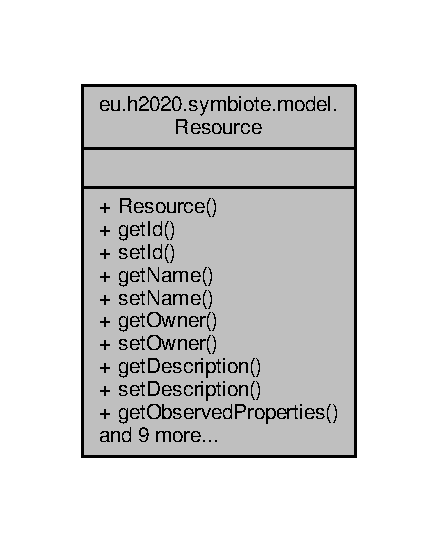
\includegraphics[width=210pt]{classeu_1_1h2020_1_1symbiote_1_1model_1_1Resource__coll__graph}
\end{center}
\end{figure}
\subsection*{Public Member Functions}
\begin{DoxyCompactItemize}
\item 
\mbox{\Hypertarget{classeu_1_1h2020_1_1symbiote_1_1model_1_1Resource_a6d2b00f0e94b55cce1daff002012369c}\label{classeu_1_1h2020_1_1symbiote_1_1model_1_1Resource_a6d2b00f0e94b55cce1daff002012369c}} 
String {\bfseries get\+Id} ()
\item 
\mbox{\Hypertarget{classeu_1_1h2020_1_1symbiote_1_1model_1_1Resource_a209815ba7cdb6b82334e664eb4c38708}\label{classeu_1_1h2020_1_1symbiote_1_1model_1_1Resource_a209815ba7cdb6b82334e664eb4c38708}} 
void {\bfseries set\+Id} (String id)
\item 
\mbox{\Hypertarget{classeu_1_1h2020_1_1symbiote_1_1model_1_1Resource_a7332986d4dfa4ca233f705659f166f2c}\label{classeu_1_1h2020_1_1symbiote_1_1model_1_1Resource_a7332986d4dfa4ca233f705659f166f2c}} 
String {\bfseries get\+Name} ()
\item 
\mbox{\Hypertarget{classeu_1_1h2020_1_1symbiote_1_1model_1_1Resource_ad2cd06bcbfa928adead9017509cc2e78}\label{classeu_1_1h2020_1_1symbiote_1_1model_1_1Resource_ad2cd06bcbfa928adead9017509cc2e78}} 
void {\bfseries set\+Name} (String name)
\item 
\mbox{\Hypertarget{classeu_1_1h2020_1_1symbiote_1_1model_1_1Resource_a0bd495e4c9a10fac6e885de268b5ad76}\label{classeu_1_1h2020_1_1symbiote_1_1model_1_1Resource_a0bd495e4c9a10fac6e885de268b5ad76}} 
String {\bfseries get\+Owner} ()
\item 
\mbox{\Hypertarget{classeu_1_1h2020_1_1symbiote_1_1model_1_1Resource_a4391365a9ef765fb9c96e8243a45fafb}\label{classeu_1_1h2020_1_1symbiote_1_1model_1_1Resource_a4391365a9ef765fb9c96e8243a45fafb}} 
void {\bfseries set\+Owner} (String owner)
\item 
\mbox{\Hypertarget{classeu_1_1h2020_1_1symbiote_1_1model_1_1Resource_ae2ce583e094c18bca236027602739049}\label{classeu_1_1h2020_1_1symbiote_1_1model_1_1Resource_ae2ce583e094c18bca236027602739049}} 
String {\bfseries get\+Description} ()
\item 
\mbox{\Hypertarget{classeu_1_1h2020_1_1symbiote_1_1model_1_1Resource_a19349909b51f43be943fcc3ebc078009}\label{classeu_1_1h2020_1_1symbiote_1_1model_1_1Resource_a19349909b51f43be943fcc3ebc078009}} 
void {\bfseries set\+Description} (String description)
\item 
\mbox{\Hypertarget{classeu_1_1h2020_1_1symbiote_1_1model_1_1Resource_a2aaf59e1be5b0c974a31e106adfa6c43}\label{classeu_1_1h2020_1_1symbiote_1_1model_1_1Resource_a2aaf59e1be5b0c974a31e106adfa6c43}} 
List$<$ String $>$ {\bfseries get\+Observed\+Properties} ()
\item 
\mbox{\Hypertarget{classeu_1_1h2020_1_1symbiote_1_1model_1_1Resource_a826dbee60cf539ffbf1a088496ac7e11}\label{classeu_1_1h2020_1_1symbiote_1_1model_1_1Resource_a826dbee60cf539ffbf1a088496ac7e11}} 
void {\bfseries set\+Observed\+Properties} (List$<$ String $>$ observed\+Properties)
\item 
\mbox{\Hypertarget{classeu_1_1h2020_1_1symbiote_1_1model_1_1Resource_a4a0c05d9007f2216c55ddc32a44f467b}\label{classeu_1_1h2020_1_1symbiote_1_1model_1_1Resource_a4a0c05d9007f2216c55ddc32a44f467b}} 
String {\bfseries get\+Resource\+U\+RL} ()
\item 
\mbox{\Hypertarget{classeu_1_1h2020_1_1symbiote_1_1model_1_1Resource_a27d7401a8087bf902fd575039d574d0c}\label{classeu_1_1h2020_1_1symbiote_1_1model_1_1Resource_a27d7401a8087bf902fd575039d574d0c}} 
void {\bfseries set\+Resource\+U\+RL} (String resource\+U\+RL)
\item 
\mbox{\Hypertarget{classeu_1_1h2020_1_1symbiote_1_1model_1_1Resource_acfb7ead093f1ed692640c99daba8fc6c}\label{classeu_1_1h2020_1_1symbiote_1_1model_1_1Resource_acfb7ead093f1ed692640c99daba8fc6c}} 
\hyperlink{classeu_1_1h2020_1_1symbiote_1_1model_1_1Location}{Location} {\bfseries get\+Location} ()
\item 
\mbox{\Hypertarget{classeu_1_1h2020_1_1symbiote_1_1model_1_1Resource_a14eba3bd0171783f32d6d4446768905d}\label{classeu_1_1h2020_1_1symbiote_1_1model_1_1Resource_a14eba3bd0171783f32d6d4446768905d}} 
void {\bfseries set\+Location} (\hyperlink{classeu_1_1h2020_1_1symbiote_1_1model_1_1Location}{Location} location)
\item 
\mbox{\Hypertarget{classeu_1_1h2020_1_1symbiote_1_1model_1_1Resource_a1e5912a2e60f0d2dcda674f26ebe871b}\label{classeu_1_1h2020_1_1symbiote_1_1model_1_1Resource_a1e5912a2e60f0d2dcda674f26ebe871b}} 
String {\bfseries get\+Feature\+Of\+Interest} ()
\item 
\mbox{\Hypertarget{classeu_1_1h2020_1_1symbiote_1_1model_1_1Resource_abcfd5b3b2e1515ca7e9eb50eeb7ed0cf}\label{classeu_1_1h2020_1_1symbiote_1_1model_1_1Resource_abcfd5b3b2e1515ca7e9eb50eeb7ed0cf}} 
void {\bfseries set\+Feature\+Of\+Interest} (String feature\+Of\+Interest)
\item 
\mbox{\Hypertarget{classeu_1_1h2020_1_1symbiote_1_1model_1_1Resource_a97e847fb787ea9fe1d16d8bd702deece}\label{classeu_1_1h2020_1_1symbiote_1_1model_1_1Resource_a97e847fb787ea9fe1d16d8bd702deece}} 
String {\bfseries get\+Platform\+Id} ()
\item 
\mbox{\Hypertarget{classeu_1_1h2020_1_1symbiote_1_1model_1_1Resource_a4f3c37b066d6e6587912fa1f1240048f}\label{classeu_1_1h2020_1_1symbiote_1_1model_1_1Resource_a4f3c37b066d6e6587912fa1f1240048f}} 
void {\bfseries set\+Platform\+Id} (String platform\+Id)
\end{DoxyCompactItemize}


\subsection{Detailed Description}
Created by jawora on 21.\+12.\+16. 

The documentation for this class was generated from the following file\+:\begin{DoxyCompactItemize}
\item 
src/main/java/eu/h2020/symbiote/model/Resource.\+java\end{DoxyCompactItemize}

\hypertarget{interfaceeu_1_1h2020_1_1symbiote_1_1repository_1_1ResourceRepository}{}\section{eu.\+h2020.\+symbiote.\+repository.\+Resource\+Repository Interface Reference}
\label{interfaceeu_1_1h2020_1_1symbiote_1_1repository_1_1ResourceRepository}\index{eu.\+h2020.\+symbiote.\+repository.\+Resource\+Repository@{eu.\+h2020.\+symbiote.\+repository.\+Resource\+Repository}}


Inheritance diagram for eu.\+h2020.\+symbiote.\+repository.\+Resource\+Repository\+:
\nopagebreak
\begin{figure}[H]
\begin{center}
\leavevmode
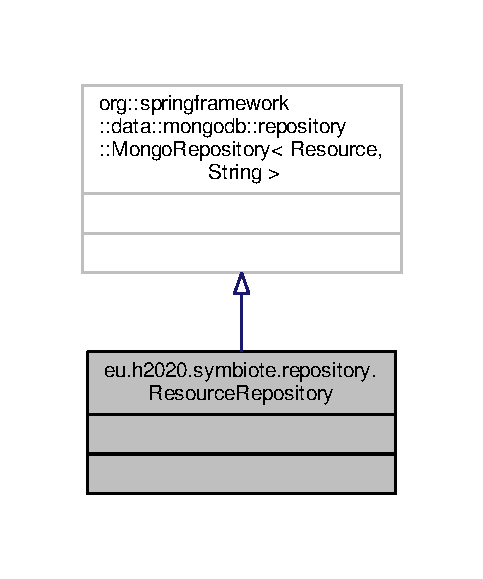
\includegraphics[width=232pt]{interfaceeu_1_1h2020_1_1symbiote_1_1repository_1_1ResourceRepository__inherit__graph}
\end{center}
\end{figure}


Collaboration diagram for eu.\+h2020.\+symbiote.\+repository.\+Resource\+Repository\+:
\nopagebreak
\begin{figure}[H]
\begin{center}
\leavevmode
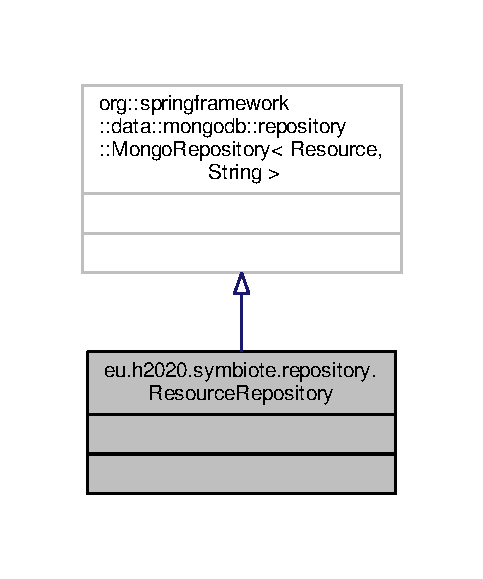
\includegraphics[width=232pt]{interfaceeu_1_1h2020_1_1symbiote_1_1repository_1_1ResourceRepository__coll__graph}
\end{center}
\end{figure}


\subsection{Detailed Description}
Created by mateuszl on 22.\+09.\+2016. 

The documentation for this interface was generated from the following file\+:\begin{DoxyCompactItemize}
\item 
src/main/java/eu/h2020/symbiote/repository/Resource\+Repository.\+java\end{DoxyCompactItemize}

\hypertarget{classeu_1_1h2020_1_1symbiote_1_1messaging_1_1RpcServer}{}\section{eu.\+h2020.\+symbiote.\+messaging.\+Rpc\+Server Class Reference}
\label{classeu_1_1h2020_1_1symbiote_1_1messaging_1_1RpcServer}\index{eu.\+h2020.\+symbiote.\+messaging.\+Rpc\+Server@{eu.\+h2020.\+symbiote.\+messaging.\+Rpc\+Server}}


Collaboration diagram for eu.\+h2020.\+symbiote.\+messaging.\+Rpc\+Server\+:
\nopagebreak
\begin{figure}[H]
\begin{center}
\leavevmode
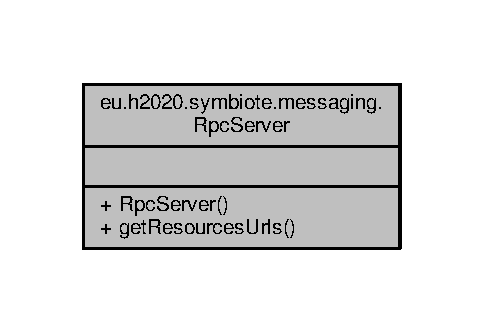
\includegraphics[width=232pt]{classeu_1_1h2020_1_1symbiote_1_1messaging_1_1RpcServer__coll__graph}
\end{center}
\end{figure}
\subsection*{Public Member Functions}
\begin{DoxyCompactItemize}
\item 
\mbox{\Hypertarget{classeu_1_1h2020_1_1symbiote_1_1messaging_1_1RpcServer_a575b7ffdc6def407b2e701f00449bc5a}\label{classeu_1_1h2020_1_1symbiote_1_1messaging_1_1RpcServer_a575b7ffdc6def407b2e701f00449bc5a}} 
{\bfseries Rpc\+Server} (\hyperlink{interfaceeu_1_1h2020_1_1symbiote_1_1repository_1_1PlatformRepository}{Platform\+Repository} platform\+Repository, \hyperlink{interfaceeu_1_1h2020_1_1symbiote_1_1repository_1_1ResourceRepository}{Resource\+Repository} resource\+Repository)
\item 
J\+S\+O\+N\+Object \hyperlink{classeu_1_1h2020_1_1symbiote_1_1messaging_1_1RpcServer_a3f4dbd0b54f371c2375215b3c13dff81}{get\+Resources\+Urls} (J\+S\+O\+N\+Object resource\+Id\+List)
\end{DoxyCompactItemize}


\subsection{Detailed Description}
\subsection*{R\+PC Server}

This listens to R\+P\+Cs from other symb\+Io\+Te Core Components via message queues.

\begin{DoxyAuthor}{Author}
Vasileios Glykantzis \href{mailto:vasgl@intracom-telecom.com}{\tt vasgl@intracom-\/telecom.\+com} 
\end{DoxyAuthor}
\begin{DoxyVersion}{Version}
1.\+0 
\end{DoxyVersion}
\begin{DoxySince}{Since}
2017-\/01-\/26 
\end{DoxySince}


\subsection{Member Function Documentation}
\mbox{\Hypertarget{classeu_1_1h2020_1_1symbiote_1_1messaging_1_1RpcServer_a3f4dbd0b54f371c2375215b3c13dff81}\label{classeu_1_1h2020_1_1symbiote_1_1messaging_1_1RpcServer_a3f4dbd0b54f371c2375215b3c13dff81}} 
\index{eu\+::h2020\+::symbiote\+::messaging\+::\+Rpc\+Server@{eu\+::h2020\+::symbiote\+::messaging\+::\+Rpc\+Server}!get\+Resources\+Urls@{get\+Resources\+Urls}}
\index{get\+Resources\+Urls@{get\+Resources\+Urls}!eu\+::h2020\+::symbiote\+::messaging\+::\+Rpc\+Server@{eu\+::h2020\+::symbiote\+::messaging\+::\+Rpc\+Server}}
\subsubsection{\texorpdfstring{get\+Resources\+Urls()}{getResourcesUrls()}}
{\footnotesize\ttfamily J\+S\+O\+N\+Object eu.\+h2020.\+symbiote.\+messaging.\+Rpc\+Server.\+get\+Resources\+Urls (\begin{DoxyParamCaption}\item[{J\+S\+O\+N\+Object}]{resource\+Id\+List }\end{DoxyParamCaption})}

Spring A\+M\+QP Listener for providing resource urls. This method is invoked when a request for access to resources is made by an aplication/enabler. Core\+Interface forwards a list of resource ids to Core\+Resource\+Access\+Monitor coming from the application/enabler and Core\+Resource\+Access\+Monitor responds with the urls of the specified resources.


\begin{DoxyParams}{Parameters}
{\em resource\+Id\+List} & The list of resource ids \\
\hline
\end{DoxyParams}
\begin{DoxyReturn}{Returns}
The urls of the resources specified in the resource\+Id\+List 
\end{DoxyReturn}


The documentation for this class was generated from the following file\+:\begin{DoxyCompactItemize}
\item 
src/main/java/eu/h2020/symbiote/messaging/Rpc\+Server.\+java\end{DoxyCompactItemize}

%--- End generated contents ---

% Index
\backmatter
\newpage
\phantomsection
\clearemptydoublepage
\addcontentsline{toc}{chapter}{Index}
\printindex

\end{document}
